%%%%%%%%%%%%%%%%%%%%%%%%%%%%%%%%%%%%%%%%%%%%%%%%%%%%%%%%%%%%%%%%%%%%%%%%%%%%%%%%%%%%%%%%%
% Section 11: Installing New Devices
%	This section provides a detailed walkthrough on how to install new devices
%	to be used in RapidSmith.
%%%%%%%%%%%%%%%%%%%%%%%%%%%%%%%%%%%%%%%%%%%%%%%%%%%%%%%%%%%%%%%%%%%%%%%%%%%%%%%%%%%%%%%%%
\newpage
\section{Installing New Device Files}
By default, the RapidSmith2 repository includes an Artix7 {\em xc7a100tcsg324}
device file. This device has been well tested, and is a good place to start if
you are learning how to use RapidSmith. However, different devices can also be created.
This section describes the necessary steps to create new device files. You need
\texttt{Tincr} installed to install new devices. 

\subsection{FamilyInfo}
A \textit{familyInfo.xml} file contains additional device information that is
not included in the XDLRC files for a given family of devices. This includes:

\begin{itemize}
  \item A list of \textbf{compatible types} for each site. Site A is said to be
  compatible with site B if the logical cells placed on site A can
  \textit{always} be placed on site B as well. For example, as shown in
  \autoref{fig:sliceCompatibility}, SLICEL sites are compatible with SLICEM
  sites. The cells placed on the SLICEL in the figure can be moved to the
  SLICEM and function indentically. SLICEM sites, however, are \textit{not}
  compatible with SLICEL sites. This is because SLICEM sites support LUT RAM
  cells, which cannot be placed on SLICEL sites.
  
  \begin{figure}[H]
    \centering
    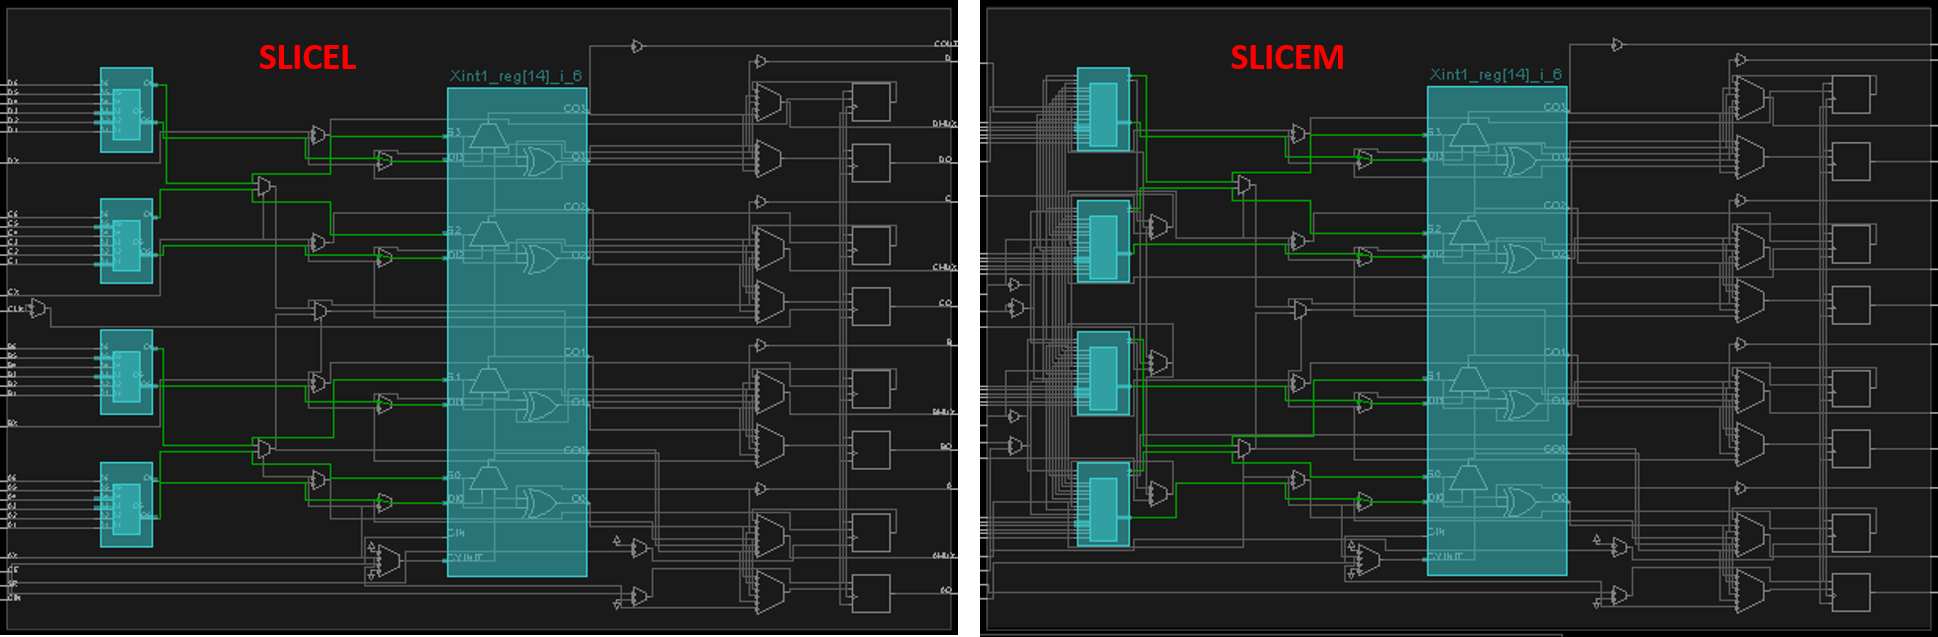
\includegraphics[width=1\columnwidth]{compatibleSites.png}
    \caption{The same group of cells placed on a SLICEL site (left) and a SLICEM
    site (right).}
    \label{fig:sliceCompatibility}
  \end{figure}
  
  \noindent Compatible sites are important
  to site-level placers in determining where a group of cells can be placed.
  \textbf{NOTE}: In some instances of compatibility, you have to first change
  the type of the compatible site before placing cells on it. For example, a
  RAMB36 site is compatible with a RAMBFIFO36 site. However, the site type of
  the RAMBFIFO36 site \textbf{must be changed to a RAMB36} type before it is
  truly compatible.
  
  \item A list of \textbf{routethrough connections} for each LUT BEL (including
  the input bel-pin and output bel-pin of the routethrough). These routethrough
  connections are turned into \texttt{Connection} objects in RapidSmith2 that
  can be used for internal site routing. Sections \ref{sec:routing} and
  \ref{sec:additionalInfo} give more information about LUT routethroughs.
  
  \item A list of \textbf{alternate types} for each site. Each physical site on
  the device has an associated default type. Some sites, however, can be
  configured to be one of many types. An example for an UltraScale
  BITSLICE\_RX\_TX site is shown in \autoref{fig:alternateTypes}. As the figure
  shows, a BITSLICE\_RX\_TX site can also be configured to be of type
  BITSLICE\_COMPONENT\_RX\_TX, BITSLICE\_RXTX\_RX, or BITSLICE\_RXTX\_TX.
  RapidSmith2 parses the alternate site information from the XML and applies it
  to the corresponding \texttt{Site} data structure. This allows users to change
  site types based on what they need.
  
    \begin{figure}[H]
    \centering
    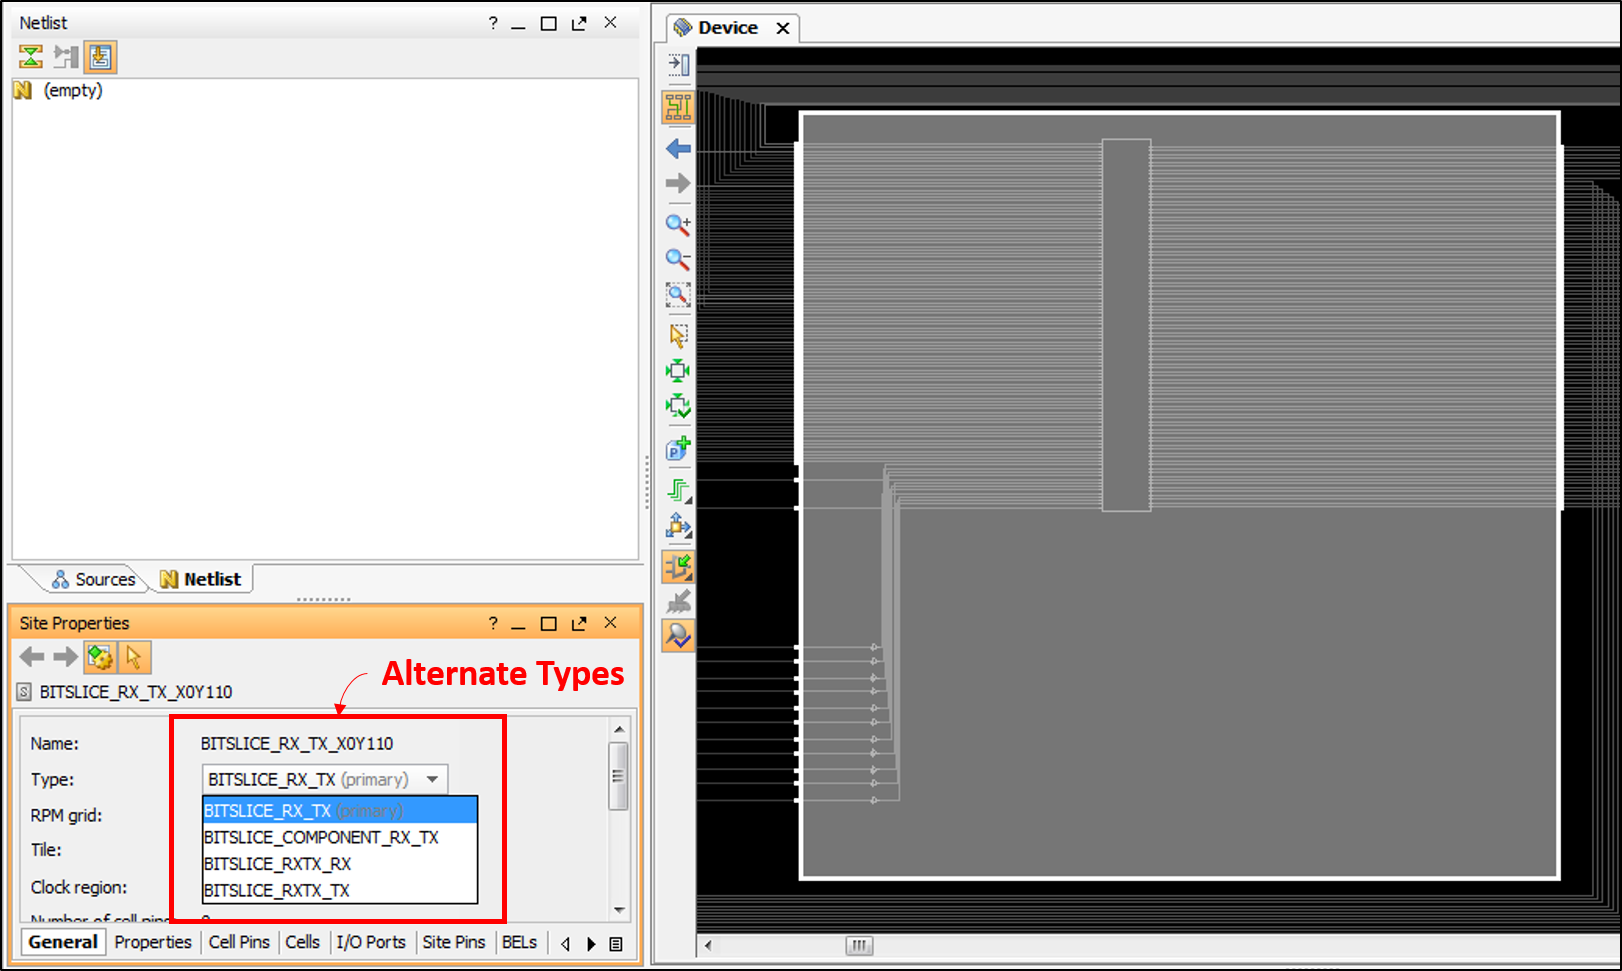
\includegraphics[width=1\columnwidth]{alternateTypes.png}
    \caption{Vivado GUI showing alternate types for a BITSLICE\_RX\_TX site.}
    \label{fig:alternateTypes}
  \end{figure}
  
  \item A list of \textbf{site pip corrections}. In the XDLRC files that are
  parsed into RapidSmith, site pips (or routing muxes) are not distinguished
  from the functional BELs (such as LUTs and Flip Flops) of a site. The
  Family Info XML identifies the site pips of a site and marks them as either
  a ``mux'' or a ``polarity\_selector.'' RapidSmith2 transforms these routing
  muxes into individual pips as shown in \autoref{fig:sitePipDecomposition} so
  that they are no longer represented as BELs. After the decomposition, each pip
  is a routing resource of the site.
  
  \begin{figure}[H]
    \centering
    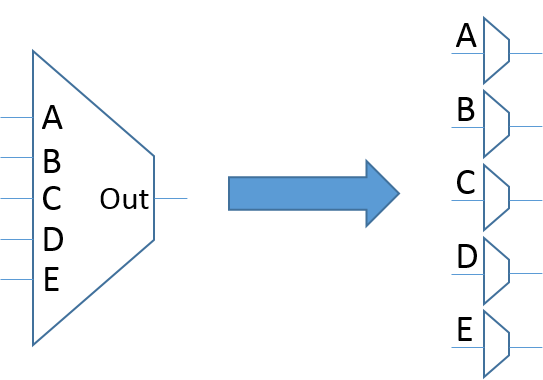
\includegraphics[width=.5\columnwidth]{sitePipDecomposition.png}
    \caption{RapidSmith2 site pip decomposition.}
    \label{fig:sitePipDecomposition}
  \end{figure}
  
  \item A list of \textbf{pin direction corrections}. For ISE-generated XDLRC
  files, all bel-pins are given a direction of either INPUT or OUTPUT. However,
  there are several bel-pins in Xilinx devices that are actually of direction
  INOUT (bidirectional). The Family Info file marks INOUT bel-pins so that
  their direction can be corrected in RapidSmith2.
  
  
\end{itemize} 
